%%%%% Projekt z předmětu IEL %%%% 
%% Autor: (doplňte)

\documentclass[]{fitiel} % dokumenty v češtině, implicitní
% \documentclass[slovak]{fitiel} % odkomentujte pro dokumenty ve slovenštině
% \documentclass[english]{fitiel} % odkomentujte pro dokumenty v angličtině
\usepackage[T1]{fontenc}
\usepackage{tgbonum}
\usepackage{caption}
%\captionsetup{justification=raggedmiddle,singlelinecheck=off}
% implicitní cesta k obrázkům
\graphicspath{{fig/}}

% hlavička 
% příkaz logo - vkládá logo fakulty dle zvoleného jazyka
\title{\logo\\IEL -- protokol k projektu}
\author{Vadim, Goncearenco \\ xgonce00}
\date{\today} % today - dnešní datum

\begin{document}
	\maketitle
	
	\tableofcontents
	
	\newpage

	%% vložení jednotlivých příkladů
	\section{Příklad 1}

% Jako parametr zadejte skupinu (A-H)
\prvniZadani{H}
\centering
\subsection{Vypočítáme $R_{ekv}$ postupným zjednodušováním obvodu}
\begin{align*}
R_{45} &= \frac{R4 \times R5}{R4 + R5} = 201,4124 \Omega
\end{align*}

\begin{figure}[H]
    \centering
    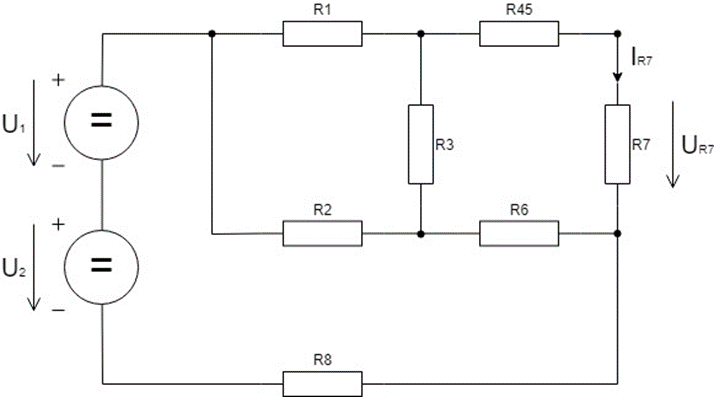
\includegraphics[width=0.6\textwidth]{fig/Pr1_1.png}
    \caption{$R_{45}~\sim~R_4,R_5$ paralelně}
    %\label{fig:mesh1}
\end{figure}

\begin{align*}
R_{457} = R_{45} + R_7 = 201,4124\Omega + 335\Omega = 536,4124\Omega
\end{align*}

\begin{figure}[H]
    \centering
    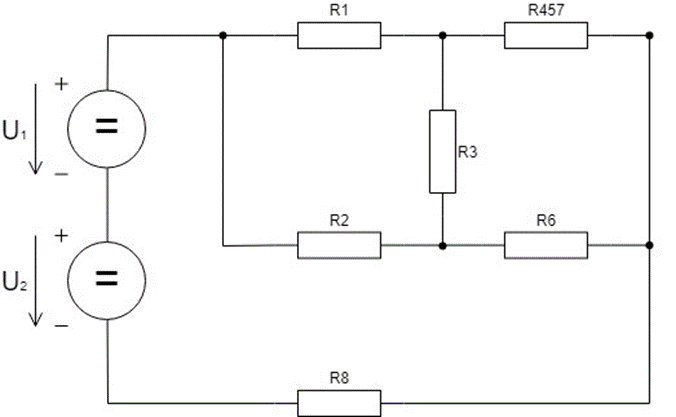
\includegraphics[width=0.6\textwidth]{fig/Pr1_2.png}
    \caption{$R_{457}~\sim~R_{45},R_7$ sériově}
    %\label{fig:mesh1}
\end{figure}

\begin{align*}
R_A &= \frac {R_1 \times R_2} {R_1 + R_2 + R_3} = \frac {408000\Omega} {1 540\Omega} = 264,9350\Omega\\
R_B &= \frac {R_1 \times R_3} {R_1 + R_2 + R_3} = \frac {176800\Omega} {1 540\Omega} = 114,8051\Omega\\
R_C &= \frac {R_2 \times R_3} {R_1 + R_2 + R_3} = \frac {156000\Omega} {1 540\Omega} = 101,2987\Omega
\end{align*}

\begin{figure}[H]
    \centering
    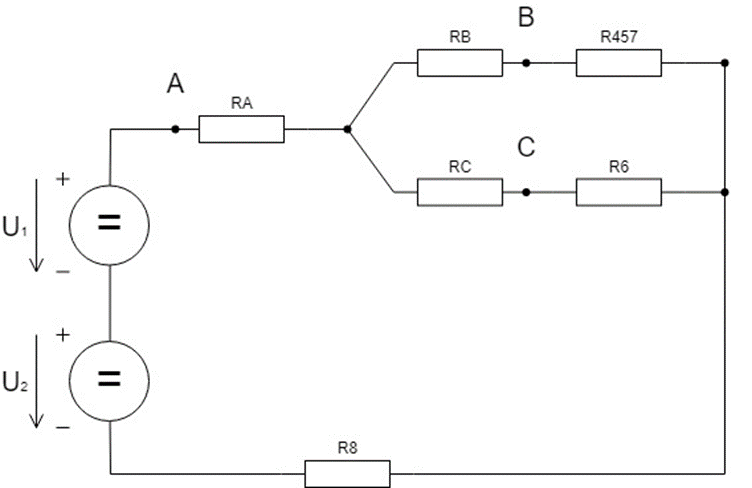
\includegraphics[width=0.6\textwidth]{fig/Pr1_3.png}
    \caption{Přechod trojúhelník $\rightarrow$ hvězda }
    %\label{fig:mesh1}
\end{figure}

\begin{align*}
R_{B457} &= R_B + R_{457} = 114,8051\Omega + 536,4124\Omega = 651,2175\Omega\\
R_{C6} &= R_C + R_6 = 101,2987\Omega + 870\Omega = 971,2987\Omega
\end{align*}

\begin{figure}[H]
    \centering
    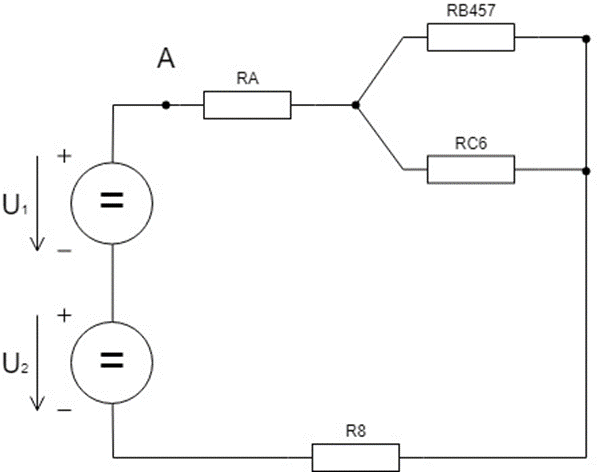
\includegraphics[width=0.6\textwidth]{fig/Pr1_4.png}
    \caption{$R_{B457}~\sim~R_B,R_{457}$ sériově,~$R_{C6}~\sim~R_C,R_6$ sériově}
    %\label{fig:mesh1}
\end{figure}

\begin{align*}
R_{B457C6} = \frac {R_{B457} \times R_{C6}} {R_{B457} + R_{C6}} = \frac {632 526,7111\Omega} {1 622,5162\Omega} = 389,8430\Omega
\end{align*}

\begin{figure}[H]
    \centering
    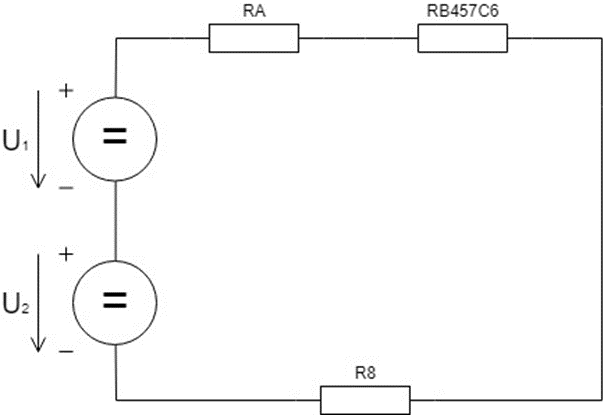
\includegraphics[width=0.6\textwidth]{fig/Pr1_5.png}
    \caption{$R_{B457C6}~\sim~R_{B457},R_{C6}$ paralelně}
    %\label{fig:mesh1}
\end{figure}

\begin{align*}
R_{AB457C6} &= R_A + R_{B457C6} = 264,9350\Omega + 389,8430\Omega = 654,778\Omega\\
R_{AB457C68} &= R_{AB457C6} + R_8 = 654,778\Omega + 265\Omega = 919,778\Omega\\
R_{ekv} &= R_{AB457C68} = 919,778\Omega
\end{align*}

\begin{figure}[H]
    \centering
    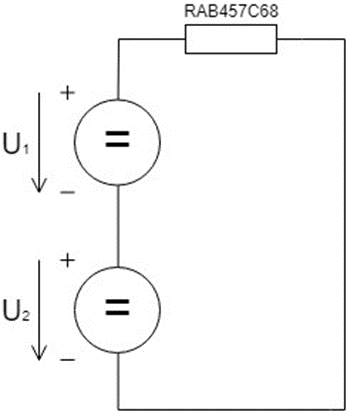
\includegraphics[width=0.3\textwidth]{fig/Pr1_6.png}
    \caption{$R_{AB457C6}~\sim~R_A,R_{B457C6}$ sériově, $R_{ekv}~\sim~R_{AB457C6},R_8$ sériově}
    %\label{fig:mesh1}
\end{figure}

\subsection{Zpětným chodem vypočítáme $U_{R7},~I_{R7}$ }

\begin{align*}
U &= U_1 + U_2 = 135V + 80V = 215 V\\
I &= \frac {U} {R_{ekv}} = \frac {215V} {919,778\Omega} = 0,2337 A\\ \\
U_{RAB457C6} &= R_{AB457C6} \times I = 654,778\Omega \times 0,2337 A = 153,0216 V\\
U_{R8} &= R_8 \times I = 265\Omega \times 0,2337 A = 61,9305 V\\ \\
U_{RA} &= R_A \times I = 264,9350\Omega \times 0,2337 A = 61,9153 V\\
U_{RB457C6} &= R_{B457C6} \times I = 389,8430\Omega \times 0,2337 A = 91,1063 V\\ \\
I_{RB457} &= \frac {U_{RB457C6}} {R_{B457}} = \frac {91,1063 V} {651,2175\Omega} = 0,1399 A\\
I_{RC6} &= \frac {U_{RB457C6}} {R_{C6}} = \frac {91,1063 V} {971,2987\Omega} = 0,0937 A
\end{align*}
\begin{align*}
U_{RB} &= R_B \times I_{RB457} = 114,8051\Omega \times 0,1399 A = 16,0612 V\\
U_{R457} &= R_{457} \times I_{RB457} = 536,4124\Omega \times 0,1399 A = 75,0440 V\\
U_{RC} &= R_C \times I_{RC6} = 101,2987\Omega \times 0,0937 A = 9,4916 V\\
U_{R6} &= R_6 \times I_{RC6} = 870\Omega \times 0,0937 A = 81,519 V
\end{align*}
\begin{figure}[H]
    \centering
    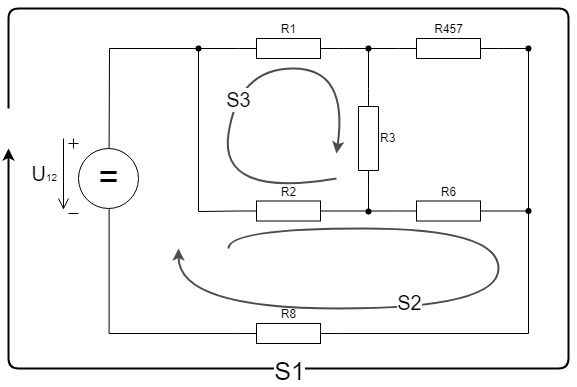
\includegraphics[width=0.6\textwidth]{fig/Pr1_7.jpg}
    \caption{Smyčka S1, S2, S3}
    %\label{fig:mesh1}
\end{figure}
\begin{align*}
S1: U_{R1} &+ U_{R457} + U_{R8} - U = 0 \textit{ (II Kir. Z)}\\
S2: U_{R2} &+ U_{R6} + U_{R8} - U = 0 \textit{ (II Kir. Z)}\\
S3: U_{R2} &- U_{R1} - U_{R3} = 0 \textit{ (II Kir. Z)}
\end{align*}
\begin{align*}
U_{R1} &= U - U_{R457} - U_{R8} = 215 V - 75,0440 V - 61,9305 V = 78,0255 V\\
U_{R2} &= U - U_{R6} - U_{R8} = 215 V - 81,519 V - 61,9305 V = 71,5505 V\\
U_{R3} &= U_{R1} - U_{R2} = 78,0255 V - 71,5505 V = 6,4750 V\\ \\
I_{R457} &= \frac {U_{R457}} {R_{457}} = \frac {75,0440 V} {536,4124\Omega} = 0,1398 A\\
I_{R457} &= \frac {U_{R45}} {R_{45}} = \frac {U_{R7}} {R_7}\\
U_{R45} &= I_{R457} \times R_{45} = 0,1398 A \times 201,4124\Omega = 28,1574 V\\ \\
\boldsymbol{U_{R7} }&=\boldsymbol{ I_{R457} \times R_7 = 0,1398 A \times 335\Omega = 46,8330 V}\\
\boldsymbol{I_{R7} }&=\boldsymbol{ I_{R457} = 0,1398 A}
\end{align*} \newpage
	\section{Příklad 2}
% Jako parametr zadejte skupinu (A-H)
\druhyZadani{C}
\subsection{Zjednodušovaní obvodu}
\begin{align*}
R_{45} = R_4 + R_5 = 240\Omega + 450\Omega = 690
\end{align*}

\begin{figure}[H]
    \centering
    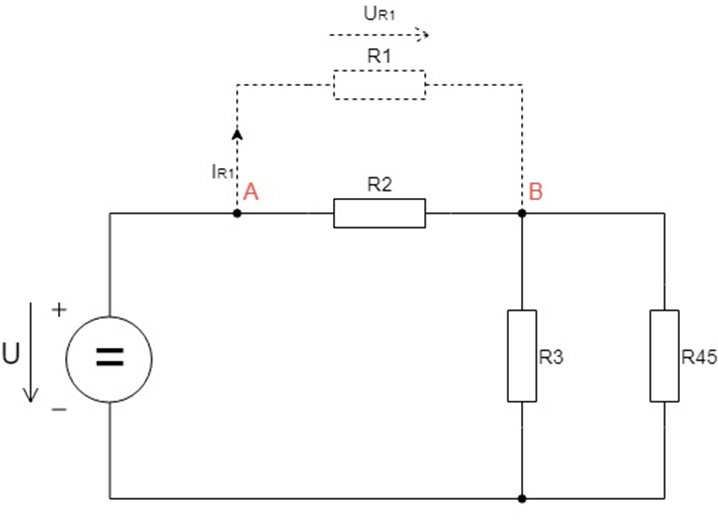
\includegraphics[width=0.6\textwidth]{fig/Pr2_1.png}
    \caption{$R_{45}~\sim~R_4,R_5$ seriove}
\end{figure}


\begin{align*}
R_{345} = \frac {R_3 \times R_{45}} {R3 + R45} = \frac {630\Omega \times 690\Omega} {630\Omega + 690\Omega} = \frac {434 700\Omega} {1320\Omega} = 329,3181\Omega
\end{align*}

\begin{figure}[H]
    \centering
    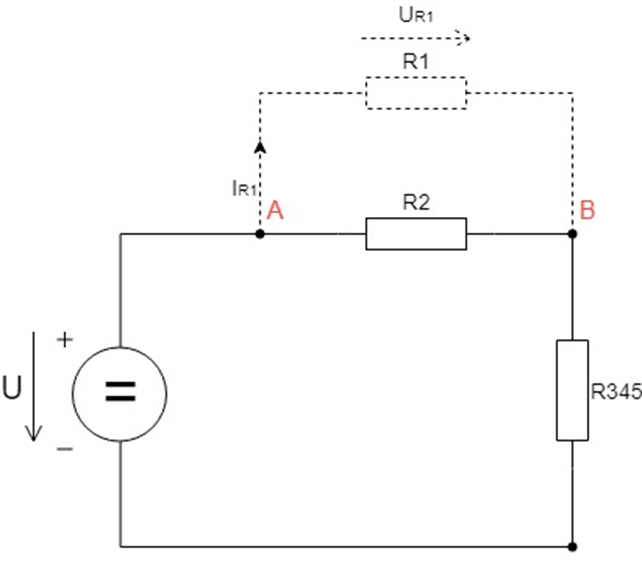
\includegraphics[width=0.6\textwidth]{fig/Pr2_2.png}
    \caption{$R_{345}~\sim~R_3,R_{45}$ parallelne}
\end{figure}
\subsection{Přechod na ekvivalentní obvod}
\begin{figure}[H]
    \centering
    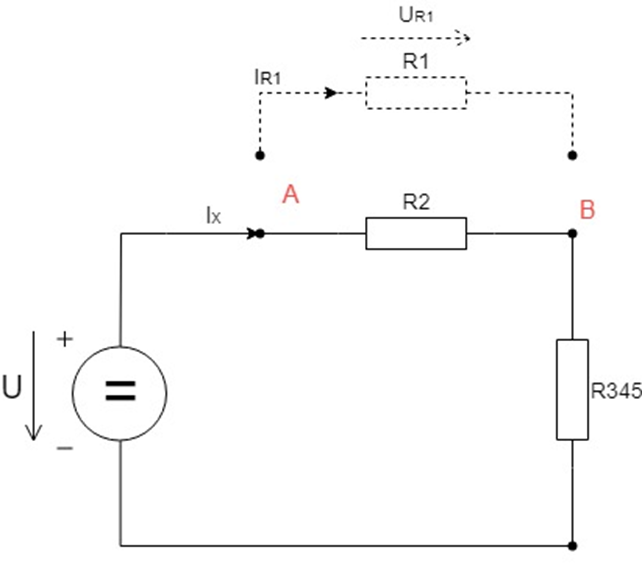
\includegraphics[width=0.6\textwidth]{fig/Pr2_3.png}
    \caption{Odpojíme větev s R1}
\end{figure}

\begin{align*}
U_i &= I_X \times R_2 + I_X \times R_{345} \textit{ (II Kir. Z.)}\\
I_X &= \frac {U} {R_2 + R_{345}} = \frac {200 V} {220\Omega + 329,3181\Omega} = \frac {200 V} {549,3181\Omega} = 0,3640 A\\
U_{AB} &= U_{R2} = I_X \times R_2 = 0,3640 A \times 220\Omega = 80,0800 V\\
R_i &= \frac {R_2 \times R_{345}} {R_2 + R_{345}} = \frac {220\Omega \times 329,3181\Omega} {220\Omega + 329,3181\Omega} = \frac {72 449,9820\Omega} {549,3181\Omega} = 131,8907\Omega\\ \\
\boldsymbol{I_{R1} }&=\boldsymbol{ \frac {U_{AB}} {R_1 + R_i} = \frac {80,0800 V} {70\Omega + 131,8907\Omega} = \frac {80,0800 V} {201,8907\Omega} = 0,3966 A}\\
\boldsymbol{U_{R1} }&=\boldsymbol{ I_{R1} \times R_1 = 0,3966 A \times 70\Omega = 27,7620 V}\\
\end{align*}

\begin{figure}[H]
    \centering
    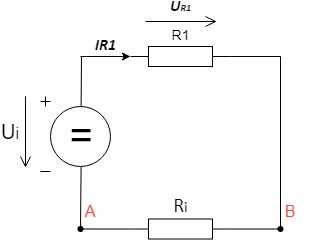
\includegraphics[width=0.4\textwidth]{fig/Pr2_4.jpg}
    \caption{Ekvivalentní obvod}
\end{figure} \newpage
	\section{Příklad 3}
% Jako parametr zadejte skupinu (A-H)
\tretiZadani{C}
\subsubsection{Zvolíme uzel D jako referenční}
\begin{align*}
U_D &= 0 V
\end{align*}
\subsubsection{Vzorce pro jednotlivé proudy}
\begin{align*}
I_{R1} &= \frac {U_A - U_D} {R_1} = \frac {U_A} {R_1}\\
I_{R2} &= \frac {U_C - U_D} {R_2} = \frac {U_C} {R_2}\\
I_{R3} &= \frac {U_B - U_C} {R_3}\\
I_{R4} &= \frac {U_A - U_B} {R_4}\\
I_{R5} &= \frac {U_B - U_A + U} {R_5}
\end{align*}
\subsubsection{I Kir. Z. pro proudy v uzlech}
\begin{align*}
&I_1 + I_{R5} - I_{R1} - I_{R4} = 0~(Uzel A.)\\
&I_{R4} + I_2 - I_{R5} - I_{R3} = 0~(Uzel B.)\\
&I_{R3} - I_2 - I_{R2} = 0~~~~~~~~~~(Uzel C.)
\end{align*}
\begin{align*}
&I_1 + \frac {U_B - U_A + U} {R_5} - \frac {U_A} {R_1} - \frac {U_A - U_B} {R_4} = 0\\
&\frac {U_A - U_B}{R_4} + I_2 - \frac {U_B - U_A + U} {R_5} - \frac {U_B - U_C} {R_3} = 0\\
&\frac {U_B - U_C} {R_3} - I_2 - \frac {U_C} {R_2} = 0
\end{align*}
\begin{align*}
-U \times G_5 - I_1 &= U_B \times (G_5 + G_4) - U_A \times (G_5 + G_1 + G_4)\\
U \times G_5 - I_2 &= U_A \times (G_4 + G_5) - U_B \times (G_4 + G_5 + G_3) + U_C \times G_3\\
I_2 &= U_B \times G_3 - U_C \times (G_3 + G_2)
\end{align*}
\subsubsection{Dosadíme hodnoty a vypočítáme napětí na uzlech}
\begin{align*}
-4.5166 A &= U_B \times \frac {1} {12\Omega} - U_A \times \frac {7} {66\Omega}\\
2.9166 A &= U_A \times \frac {1} {12\Omega} - U_B \times \frac {17} {168\Omega} + U_C \times \frac {1} {56\Omega}\\
0.75 A &= U_B \times \frac {1} {56\Omega} - U_C \times \frac {87} {1736\Omega}
\end{align*}
\begin{align*}
U_A &= 52.3536 V\\
U_B &= 12.4327 V\\
U_C &= -10.5355 V
\end{align*}
\subsubsection{Vypočítáme napětí a proud na rezistoru $R_3$}
\begin{align*}
U_{R3} &= U_B - U_C = 22.9656 V\\
I_{R3} &= \frac {U_{R3}} {R_3} = 0.4101 A
\end{align*} \newpage
	\section{Příklad 4}
% Jako parametr zadejte skupinu (A-H)
\ctvrtyZadani{H}
\subsubsection{Vzorce pro impedanci a uhlovou frekvenci}
\begin{align*}
\omega &= 2 \pi f\\
Z_C &= \frac{-j}{\omega C}\\
Z_L &= j \omega L
\end{align*}
\subsubsection{II Kir. Z. pro rovnice proudu ve smyčkách}
\begin{align*}
I_A &: U_{L1} + U_1 + U_{C2} + U_{R1} = 0\\
I_B &: U_{R1} + U_2 + U_{C1} = 0\\
I_C &: U_{C2} + U_{L2} + U_{R2} - U_2 = 0
\end{align*}
\begin{align*}
I_A &: I_A (Z_{L1} + Z_{C2} + R_1) - I_BR_1 - I_CZ_{C2}\\
I_B &: I_B (R_1 + Z_{C1}) - I_AR_1 = -U_2\\
I_C &: I_C (Z_{C2} + Z_{L2} + R_2) - I_A Z_{C2} = U_2
\end{align*}
\subsubsection{Výpočet proudu pomoci matic}
\centering
\begin{align*}
    \begin{pmatrix}
    Z_{L1} + Z_{C2} + R_1 & -R_1 & -Z_{C2}\\
    -R_1 & R_1 + Z_{C1} & 0\\
    -Z_{C2} & 0 & Z_{C2} + Z_{L2} + R_2
    \end{pmatrix}
    \times
    \begin{pmatrix}
    I_A\\
    I_B\\
    I_C
    \end{pmatrix}
    &=
    \begin{pmatrix}
    -U_1\\
    -U_2\\
    U_2\\
    \end{pmatrix}
    \\ \\
    \begin{pmatrix}
    10 + 71.5713j & -10 & 23.9391\\
    -10 & 10 - 10.8085j & 0\\
    23.9331j & 0 & 10 + 20.8346j
    \end{pmatrix}
    \times
    \begin{pmatrix}
    I_A\\
    I_B\\
    I_C
    \end{pmatrix}
    &=
    \begin{pmatrix}
    -5\\
    -6\\
    6
    \end{pmatrix}
\end{align*}
\subsubsection{Násobením inverzní matici zleva dostáváme hodnoty proudu}
\begin{align*}
I_A &= (-0.2105 + 0.2255j) A\\
I_B &= (-0.4862 - 0.3j) A\\
I_C &= (0.4099 - 0.3502j) A
\end{align*}
\subsubsection{Formuli pro napětí a fázový posun L2}
\begin{align*}
U_{L2} &= I_C \times Z_{L2}\\
\vert U_{L2}\vert &= \sqrt{ re(U_{L2})^2 + im(U_{L2})^2 }
\end{align*}
\begin{align*}
\varphi &= atan(\frac {im(U_{L2})}{re(U_{L2})})
\end{align*}
\centering
\subsubsection{Dosadíme hodnoty do vzorců}
\begin{align*}
I_{L2} &= I_C = (0.4099 - 0.3502j) A\\
U_{L2} &= I_{L2}\times Z_{L2} = (0.4099 - 0.3502j) A \times (0 + 44.7676j) A = (15.6810 + 18.3519j) V\\ \\
\boldsymbol{\varphi }&=\boldsymbol{ atan(\frac {im(U_{L2})}{re(U_{L2})}) = atan(\frac {18.3519}{15.6810})  = 0.8637^{~\circ}}\\
\boldsymbol{\vert U_{L2}\vert }&=\boldsymbol{ \sqrt{ re(U_{L2})^2 + im(U_{L2})^2 } = \sqrt{15.6810^2 + 18.3519^2} = 24.1389 V}
\end{align*} \newpage
	\section{Příklad 5}
% Jako parametr zadejte skupinu (A-H)
\patyZadani{C}
\subsubsection{Vzorec pro napětí na kondenzátoru}
\begin{align*}
U_C’ &= \frac{I}{C}
\end{align*}
\subsubsection{II Kir. Z. pro obvod}
\begin{align*}
U_R + U_C - U &= 0
\end{align*}
\subsubsection{Algebraické úpravy}
\begin{align*}
U_C’ &= \frac{U_R}{RC}\\
U_R &= U - U_C\\
U_C’ &= \frac{U - U_C}{RC}\\
\boldsymbol{RC}&\times \boldsymbol{U_C’ + U_C = U}\\
150 &\times  U_C’ + U_C = 45
\end{align*}
\subsubsection{Očekávané řešeni}
\begin{align*}
\boldsymbol{U_C(t) }&=\boldsymbol{ k(t) \times  e^{\lambda t} }\\
\end{align*}
\subsubsection{Najdeme $\lambda$}
\begin{align*}
(U_C‘ &= \lambda; U_C = 1)\\
0 &= 150\times \lambda + 1\\
\lambda &= - \frac{1}{150}
\end{align*}
\subsubsection{Dosadíme $\lambda$ do vzorce a najdeme $k'(t)$}
\begin{align*}
U_C(t) &= k(t) \times  e^{-\frac{t}{150} }
\end{align*}
\subsubsection{Derivujeme $U_C(t)$ a najdeme $k'(t)$}
\begin{align*}
U_C’(t) &= k’(t) \times  e^{-\frac{t}{150} } - \frac {1}{150} \times  k(t) \times  e^{-\frac{t}{150}}\\
45 &= 150k’(t) \times  e^{-\frac{t}{150}}\\
k’(t) &= \frac {3}{10} \times  e^{\frac{t}{150}}
\end{align*}
\subsubsection{Integrujeme $k'(t)$ a dosadíme do vzorce pro $U_C(t)$}
\begin{align*}
k(t) = \int \frac {3}{10} \times  e^{\frac{t}{150}} dt &= \frac{3}{10} \times 150 \times e^{\frac{t}{150}} = 45 \times  e^{\frac{t}{150}} + C\\
U_C(t) &= (45 \times e^{\frac{t}{150}} + C) \times  e^{-\frac{t}{150}}\\
\boldsymbol{U_C(t) }&=\boldsymbol{ 45 + C \times  e^{-\frac{t}{150}} }
\end{align*}
\subsubsection{Najdeme C}
\begin{align*}
U_C(0) &= 45 + C\\
12 &= 45 + C\\
C &= -33\\ \\
\boldsymbol{U_C(t) }&=\boldsymbol{ 45 - 33 \times  e^{-\frac{t}{150}} }
\end{align*} \newpage
	
	%% vložení tabulky s přehledem výsledků
	\section{Shrnutí výsledků}
    \begin{tabular}{|c|c|c|} \hline 
        \textbf{Příklad} & \textbf{Skupina} & \textbf{Výsledky} \\ \hline
        1 & \prvniSkupina & $U_{R7} = 46,8330 V$ \qquad \qquad $I_{R7} = 0,1398 A$ \\ \hline
        2 & \druhySkupina & $U_{R1} = 27,7620 V$ \qquad \qquad $I_{R1} = 0,3966 A$ \\ \hline
        3 & \tretiSkupina & $U_{R3} = 22.9656 V$ \qquad \qquad $I_{R3} = 0.4101 A$\\ \hline
        4 & \ctvrtySkupina & $|U_{L_{2}}| = 24.1389 V$ \qquad \qquad $\varphi_{L_{2}} = 0.8637^{\circ}$ \\ \hline
        5 & \patySkupina & $u_C = 45 - 33 \times  e^{-\frac{t}{150}}$ \\ \hline
    \end{tabular}

	
\end{document}
